% Adjust these for the path of the theme and its graphics, relative to this file
%\usepackage{beamerthemeFalmouthGamesAcademy}
\usepackage{../../beamerthemeFalmouthGamesAcademy}
\usepackage{multimedia}
\graphicspath{ {../../} }

% Default language for code listings
\lstset{language=C++,
        morekeywords={each,in,nullptr}
}

% For strikethrough effect
\usepackage[normalem]{ulem}
\usepackage{wasysym}

\usepackage{pdfpages}

\begin{document}
\title{Smart Pointers}   
\subtitle{COMP110: Principles of Computing}

\frame{\titlepage} 

%\begin{frame}{Today's lecture}
    %Today's lecture has \textbf{three parts}
    %\begin{itemize}
        %\item Software testing and test-driven development
        %\item Introducing COMP110 Coding Task II
        %\item Object composition in C++
    %\end{itemize}
%\end{frame}
%
\part{Statics and singletons}
\frame{\partpage}

\begin{frame}{Static members}
    \begin{itemize}
        \item Class members (methods and fields) can be marked as \lstinline{static} \pause
        \item They are then \textbf{shared} across \textbf{all instances} of the class \pause
        \item Static members can be accessed from \textbf{outside} the class using \lstinline{::} notation
    \end{itemize}
\end{frame}

\begin{frame}[fragile]{The singleton pattern}
    \begin{itemize}
        \item A \textbf{singleton} class has a \textbf{single static instance} \pause
        \item A \textbf{static} \lstinline{getInstance} function returns a \textbf{reference} to the instance \pause
        \item There is \textbf{one and only one} instance --- creating new instances is not allowed,
            neither is destroying the existing instance
    \end{itemize}
\end{frame}

\begin{frame}[fragile]
    In \texttt{TextureManager.h}
    \begin{lstlisting}
class TextureManager
{
public:
    static TextureManager& getInstance()
    { return instance; }
    
    Texture* getTexture(const std::string& name);
    
private:
    TextureManager() { };
    static TextureManager instance;
};
    \end{lstlisting} \pause
    In \texttt{TextureManager.cpp}
    \begin{lstlisting}
#include "TextureManager.h"

TextureManager TextureManager::instance;
    \end{lstlisting}
\end{frame}

\begin{frame}[fragile]
    Key points: \pause
    \begin{itemize}
        \item Constructor is \textbf{private} to prevent creation of extra instances \pause
        \item \lstinline{instance} and \lstinline{getInstance} are \textbf{static}, everything else is \textbf{not static} \pause
        \item Static variables must be \textbf{instantiated} in a \texttt{.cpp} file
            \begin{itemize}
                \item Optionally with constructor parameters
            \end{itemize} \pause
    \end{itemize}
    Example usage:
    \begin{lstlisting}
Texture* texture = TextureManager::getInstance().getTexture("player.png");
    \end{lstlisting}
\end{frame}

\begin{frame}[fragile]{Statics and initialisation}
    \begin{itemize}
        \item Static members are initialised at the \textbf{very start of the program} \pause
            \begin{itemize}
                \item I.e.\ \textbf{before} \lstinline{main()} is entered \pause
            \end{itemize}
        \item The order of initialisation is \textbf{undefined} \pause
            \begin{itemize}
                \item \textbf{Do not} make your static initialisation code rely on other statics having been initialised already ---
                    this \textbf{will} cause obscure bugs! \pause
            \end{itemize}
        \item Further reading: \url{https://isocpp.org/wiki/faq/ctors#static-init-order} \pause
        \item Consider using the \textbf{construct on first use} idiom if your singleton class
            has a complex constructor
    \end{itemize}
\end{frame}


%\part{Smart pointers}
%\frame{\partpage}

\begin{frame}{Motivation}
    \begin{itemize}
        \item Pointers in C++ are powerful, but with great power comes great responsibility!
        \item In particular, responsibility for the \textbf{lifetime} of object instances,
            i.e.\ remembering to call \lstinline{delete} at the right time
        \item C++11 introduced \textbf{smart pointers} to try and make this easier
    \end{itemize}
\end{frame}

\begin{frame}{Unique pointer}
    \begin{itemize}
        \item Defined in standard header file \lstinline{<memory>}
        \item \lstinline{std::unique_ptr} has \textbf{sole ownership} of the instance to which it points
        \item I.e.\ two \lstinline{unique_ptr}s \textbf{cannot} point to the same instance
        \item Use \lstinline{std::make_unique<T>} instead of \lstinline{new T}
        \item The instance is destroyed when the \lstinline{unique_ptr} goes \textbf{out of scope},
            or when it is assigned to point to a different instance
    \end{itemize}
\end{frame}

\begin{frame}[fragile]{Unique pointer example}
    \begin{lstlisting}
#include "stdafx.h" // --> #include <memory>

class MyClass { };

int main()
{
    std::unique_ptr<MyClass> p
        = std::make_unique<MyClass>();
    return 0;
    // p is automatically deleted here
}
    \end{lstlisting}
\end{frame}

\begin{frame}[fragile]{Aside: automatic type inference}
    \begin{itemize}
        \item When declaring a \textbf{local variable} with an initial value,
            can use \lstinline{auto} in place of the type
        \item The compiler \textbf{infers} the type from the type of the initial value
    \end{itemize}
    \begin{lstlisting}
// The following are equivalent:
std::unique_ptr<Duck> duck = std::make_unique<Duck>();
auto duck = std::make_unique<Duck>();
    \end{lstlisting}
    \begin{itemize}
        \item Careful --- this can make your code \textbf{more readable} or \textbf{less readable}
            depending on how and where you use it!
    \end{itemize}
\end{frame}

\begin{frame}{Vectors of objects revisited}
    From last time:
    \begin{itemize}
        \item \lstinline{std::vector<Duck>}: when the vector changes size, instances are 
            \textbf{copied} and the old ones \textbf{destroyed}
        \item \lstinline{std::vector<Duck*>}: no copying and destroying, but you must
            remember to \lstinline{delete} elements on removal
    \end{itemize}
    But now:
    \begin{itemize}
        \item \lstinline{std::vector<std::unique_ptr<Duck>>}: class instances stay put,
            but are automatically destroyed when removed from the \lstinline{vector}!
    \end{itemize}
\end{frame}

\begin{frame}[fragile]{Unique pointers can't be copied}
    \begin{lstlisting}
auto p = std::make_unique<MyClass>();
auto q = p;
    \end{lstlisting}
    \begin{itemize}
        \item This won't compile!
    \end{itemize}
    
\includegraphics[width=\textwidth]{unique_ptr_error}
    \begin{itemize}
        \item Translation: assigning one \lstinline{unique_ptr} from another is forbidden
    \end{itemize}
\end{frame}

\begin{frame}[fragile]{Unique pointers can be moved}
    \begin{lstlisting}
auto p = std::make_unique<MyClass>();
auto q = std::move(p);
    \end{lstlisting}
    \begin{itemize}
        \item Now \lstinline{q} has \textbf{ownership} of the instance
        \item \lstinline{p} no longer refers to this instance
        \item In fact \lstinline{p} becomes null
        \item Another way you are allowed to move \lstinline{unique_ptr}s is bu \textbf{swapping}:
    \end{itemize}
    \begin{lstlisting}
auto p = std::make_unique<MyClass>("hello");
auto q = std::make_unique<MyClass>("world");
std::swap(p, q);
    \end{lstlisting}
\end{frame}

\begin{frame}{Shared pointers}
    \begin{itemize}
        \item Unique pointers have their uses, but uniqueness is a big restriction
        \item C++ also has \lstinline{std::shared_ptr}, which does allow multiple pointers to the same
            instance
        \item \textbf{Reference counting} ensures the instance is destroyed when
            \textbf{all \lstinline{shared_ptr}s} to it have gone away
    \end{itemize}
\end{frame}

\begin{frame}[fragile]
    \begin{lstlisting}
int main()
{
	bool flag = true;
	std::shared_ptr<MyClass> p = nullptr;
	
	if (flag)
	{
		auto q = std::make_shared<MyClass>();
		p = q;
	}
    /* q is out of scope, but p still holds a reference to the instance so it stays alive */
    
    if (p)
        p->doSomething();
    
    return 0;
    /* p is out of scope now, so the instance is destroyed */
}
    \end{lstlisting}
\end{frame}

\begin{frame}{Reference counting}
    \begin{itemize}
        \item Objects managed by \lstinline{shared_ptr} have a \textbf{reference count}, initially 0
        \item When a \lstinline{shared_ptr} is made to point to the instance,
            its reference count is \textbf{incremented}
        \item When a \lstinline{shared_ptr} no longer points to the instance
            (because it goes out of scope or is reassigned),
            the reference count is \textbf{decremented}
        \item When the reference count is decremented to 0,
            the instance is destroyed
    \end{itemize}
\end{frame}

\begin{frame}{Smart pointers and composition}
    \begin{itemize}
        \item We have seen \lstinline{unique_ptr} and \lstinline{shared_ptr} used as
            \textbf{local variables}
        \item They can also be used as \textbf{fields} within classes
        \item When the instance containing them is destroyed:
            \begin{itemize}
                \item \lstinline{unique_ptr} destroys the instance to which it points
                \item \lstinline{shared_ptr} decrements the reference count on the instance 
                    to which it points, which may result in it being destroyed
            \end{itemize}
        \item ... just as you would expect (hopefully)!
    \end{itemize}
\end{frame}

\begin{frame}[fragile]
    \begin{lstlisting}
class Duck
{
public:
    Duck(const std::shared_ptr<Pond>& pond)
        : pond(pond),
          bill(std::make_unique<Bill>())
    { }
    
private:
    std::unique_ptr<Bill> bill;
    std::shared_ptr<Pond> pond;
};
    \end{lstlisting}
    When a \lstinline{Duck} instance is destroyed:
    \begin{itemize}
        \item Its \lstinline{Bill} is also destroyed;
        \item Its \lstinline{Pond} is destroyed \textbf{if and only if} there are no other
            \lstinline{shared_ptr}s to it (e.g.\ in other \lstinline{Duck} instances)
    \end{itemize}
\end{frame}

\begin{frame}[fragile]
    \begin{lstlisting}
class Bar;

class Foo
{
public:
    std::shared_ptr<Bar> bar;
};

class Bar
{
public:
    std::shared_ptr<Foo> foo;
};

int main()
{
    auto p = std::make_shared<Foo>();
    p->bar = std::make_shared<Bar>();
    p->bar->foo = p;
}
    \end{lstlisting}
\end{frame}

\begin{frame}{Reference cycles}
    \begin{itemize}
        \item In the example on the previous slide,
            the instances are \textbf{not} destroyed properly at the end of \lstinline{main()}
        \item \lstinline{Foo} still holds a reference to \lstinline{Bar},
            but \lstinline{Bar} holds a reference to \lstinline{Foo}
        \item This prevents both objects' reference counts from reaching 0
        \item Solution: make one of the references a \textbf{weak pointer}
    \end{itemize}
\end{frame}

\begin{frame}[fragile]{Weak pointers}
    \begin{itemize}
        \item \lstinline{std::weak_ptr} is similar to \lstinline{std::shared_ptr},
            except it does \textbf{not} alter the reference count of the instance
        \item A \lstinline{weak_ptr} must be \textbf{locked} in order to access the instance to which
            it points
    \end{itemize}
    \begin{lstlisting}
std::shared_ptr<MyClass> lockedInstance
    = weakPtr.lock();
    \end{lstlisting}
    \begin{itemize}
        \item Locking creates a temporary \lstinline{shared_ptr} to the instance ---
            this ensures that the reference count stays above 0 while the instance is being used
    \end{itemize}
\end{frame}

\begin{frame}[fragile]{Smart pointers --- Summary}
    \begin{itemize}
        \item \lstinline{std::shared_ptr} uses \textbf{reference counting} to manage the lifetime
            of objects
        \item \lstinline{std::weak_ptr} is useful for breaking \textbf{reference cycles}
            when using \lstinline{shared_ptr}s for composition
        \item \lstinline{std::unique_ptr} can be used when you want to enforce that there is
            \textbf{only one} pointer to a particular instance
        \item NB: all smart pointer types allow \textbf{polymorphism}, e.g.
    \end{itemize}
    \begin{lstlisting}
class Bird {};
class Duck : public Bird {};

std::shared_ptr<Bird> bird = std::make_unique<Duck>();
    \end{lstlisting}
\end{frame}

\begin{frame}[fragile]{What about ``dumb'' pointers?}
    \begin{itemize}
        \item In modern C++, it is \textbf{almost always preferable} to use smart pointers
            instead of normal C++ pointers
        \item I.e.\ use \lstinline{std::make_unique} / \lstinline{std::make_shared} instead of
            \lstinline{new}, and then you never have to worry about calling \lstinline{delete}
        \item So why did we bother teaching you about normal C++ pointers?!
            \begin{itemize}
                \item Because C++ code written before 2011 (and much code written after) uses them extensively
                \item Because sometimes you need to use them,
                    e.g.\ when working with SDL or other APIs / libraries
                \item Because once you understand pointers, you can call yourself a Real Programmer \smiley
            \end{itemize}
    \end{itemize}
\end{frame}


\part{Admin and Etiquette}
\frame{\partpage}

\begin{frame}{Attendance}
    \begin{center}
        Please mark yourself as present on the attendance system!
    \end{center}
\end{frame}

\begin{frame}{Teams Etiquette}
    \begin{itemize}
        \pause\item This session is a \textbf{Live Event} --- you can't unmute, but you can post in the Q\&A chat
        \pause\item Please don't post memes or spam to the chat during a session, treat it like a \textbf{professional environment}
        \pause\item If you disrupt the meeting in any way, you will be removed. You will also be reported to the Course Leader and Director of the Games Academy
    \end{itemize}
\end{frame}

% \begin{frame}{Teams Meeting Etiquette}
%     \begin{itemize}
%         \pause\item Please stay on \textbf{mute} during the Meeting
%         \pause\item \textbf{Raise your hand} if you have a question, then \textbf{unmute} when the lecturer calls on you to ask
%         \pause\item Once you have asked your question and had your question answered, please \textbf{mute} again
%         \pause\item If you don't feel comfortable talking in the meeting, please use the \textbf{chat}
%     \end{itemize}
% \end{frame}

\begin{frame}{Induction Materials}
    \begin{itemize}
        \pause\item Have you gone through all the induction materials on the COMP110 LearningSpace?
        \pause\item If not, please do so ASAP after this session!
        \pause\item Particularly important:
        \begin{itemize}
            \pause\item Module welcome video
            \pause\item Module induction video
            \pause\item Worksheet 1 brief and video
        \end{itemize}
    \end{itemize}
\end{frame}



% -------------------------------------------------------

%\part{The compiler}
%\frame{\partpage}
%
%\begin{frame}
%	\frametitle{The build process}
%	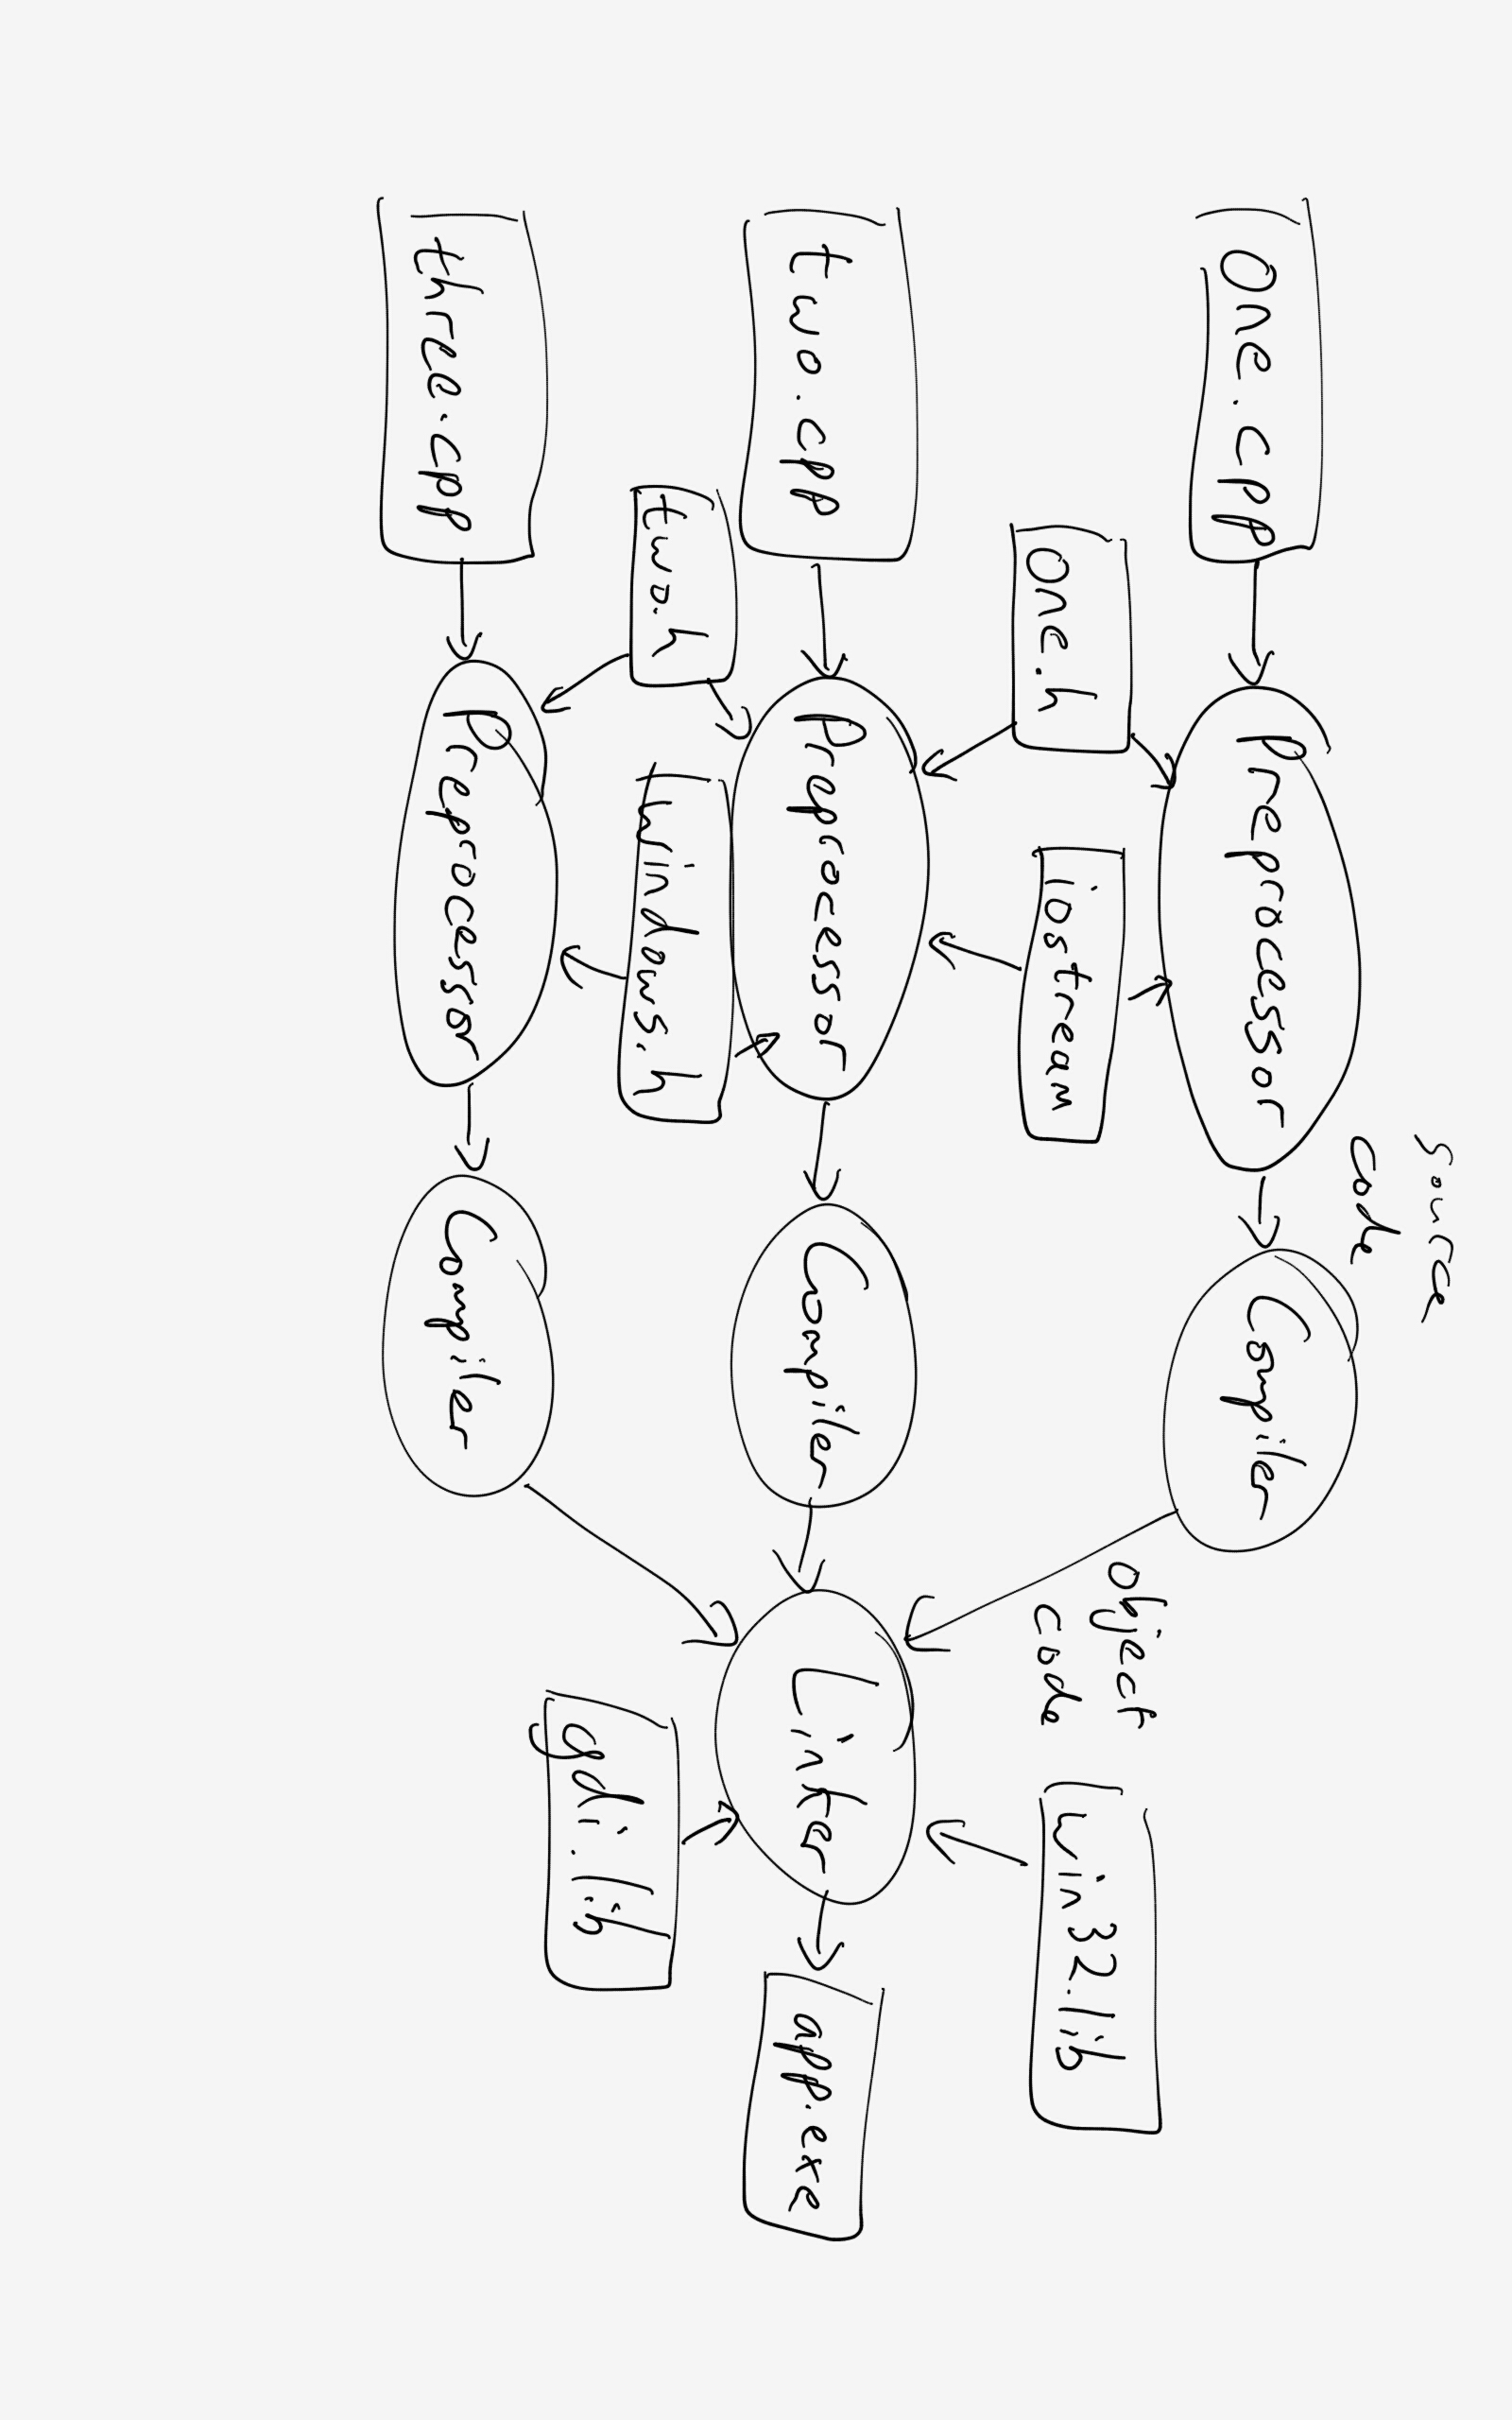
\includegraphics[height=\textwidth,angle=90]{compiler_sketch}
%\end{frame}

\end{document}
